\documentclass[10pt,a4paper]{article}
\usepackage{geometry}
\geometry{a4paper, margin=15mm, top=16mm, bottom=16mm}
\usepackage{fontspec}
\setmainfont{Noto Sans}
\newfontfamily\arabicfont{Noto Sans Arabic}[Script=Arabic]

\usepackage{tikz}
\usetikzlibrary{shapes.geometric, arrows.meta, positioning, fit, backgrounds, calc}
\usepackage{xcolor}
\usepackage{booktabs}
\usepackage{tabularx}
\usepackage{array}
\usepackage{fancyhdr}
\usepackage{tcolorbox}
\tcbuselibrary{skins, breakable}

% Professional Color Palette
\definecolor{primarynavy}{RGB}{18, 42, 80}
\definecolor{accentblue}{RGB}{32, 85, 155}
\definecolor{darkcrimson}{RGB}{150, 25, 25}
\definecolor{forestgreen}{RGB}{25, 105, 55}
\definecolor{amberbrown}{RGB}{145, 80, 10}
\definecolor{slateborder}{RGB}{195, 205, 220}
\definecolor{slatebg}{RGB}{246, 248, 251}
\definecolor{cardbg}{RGB}{255, 255, 255}
\definecolor{subtleblue}{RGB}{240, 246, 255}
\definecolor{subtlered}{RGB}{255, 242, 242}
\definecolor{subtlegreen}{RGB}{242, 252, 245}

% Must be loaded last for proper RTL rendering
\usepackage{bidi}

% Fancyhdr Setup
\pagestyle{fancy}
\fancyhf{}
\renewcommand{\headrulewidth}{0.4pt}
\renewcommand{\footrulewidth}{0.4pt}
\fancyhead[L]{\footnotesize\color{gray!80}\textbf{Project 16} $\cdot$ Natural Language Processing Lab}
\fancyhead[R]{\footnotesize\color{gray!80}Algerian Dialect Addiction Support Assistant}
\fancyfoot[L]{\footnotesize\color{gray!70}System Architecture \& Data Delivery Pipeline Specification}
\fancyfoot[R]{\footnotesize\color{gray!70}Page \thepage\ of 3}

\tikzset{
  base/.style = {rectangle, rounded corners=2.5pt, align=center, line width=0.8pt},
  flow_box/.style = {base, draw=slateborder, fill=cardbg, minimum height=0.85cm, font=\small},
  pre_box/.style = {base, draw=accentblue!70, fill=cardbg, text width=4.8cm, minimum height=0.82cm, font=\small},
  triage_box/.style = {base, draw=amberbrown!80, fill=amberbrown!5, text width=8.5cm, minimum height=0.9cm, font=\small},
  crisis_box/.style = {base, draw=darkcrimson!80, fill=cardbg, text width=5.8cm, minimum height=0.88cm, font=\small},
  rag_box/.style = {base, draw=accentblue!80, fill=cardbg, text width=7.4cm, minimum height=0.85cm, font=\small},
  output_box/.style = {base, draw=forestgreen!85, fill=subtlegreen, text width=13.5cm, minimum height=0.95cm, font=\small},
  subgraph/.style = {draw=gray!40, fill=gray!3, rounded corners=5pt, inner sep=7pt, line width=0.6pt},
  arr/.style = {-{Stealth[length=2.2mm, width=1.8mm]}, line width=0.9pt, color=gray!70},
  danger_arr/.style = {-{Stealth[length=2.2mm, width=1.8mm]}, line width=1.0pt, color=darkcrimson},
  safe_arr/.style = {-{Stealth[length=2.2mm, width=1.8mm]}, line width=1.0pt, color=primarynavy}
}

\begin{document}

% ==============================================================================
% PAGE 1: SYSTEM ARCHITECTURE SPECIFICATION
% ==============================================================================

\begin{center}
  {\Large\bfseries\color{primarynavy} Project 16: Algerian Dialect Conversational Assistant for Drug Addiction Intervention}\\[1.5mm]
  {\normalsize\bfseries\color{accentblue} System Architecture, Data Delivery Pipeline, and Operational Principles}\\[1.5mm]
  {\footnotesize\color{gray!80} Technical Design Specification $\cdot$ Dual-Engine Grounded Conversational Framework}
\end{center}

\vspace{1mm}
\noindent\rule{\textwidth}{0.6pt}
\vspace{1.5mm}

\begin{tcolorbox}[colback=slatebg, colframe=slateborder, boxrule=0.5pt, arc=3pt, left=8pt, right=8pt, top=5pt, bottom=5pt]
\footnotesize
\textbf{Executive System Objective:} This project designs and evaluates an evidence-grounded, culturally resonant conversational agent capable of interacting in Algerian Darija (spanning Arabic script, Arabizi, and Franco-Arabe code-switching). The agent provides non-judgmental guidance for individuals and family members affected by substance use disorders, combining a cross-lingual dense retrieval mechanism (RAG) with a fine-tuned dialectal language model, protected by an upstream deterministic safety triage gate.
\end{tcolorbox}

\vspace{2mm}
\noindent{\large\bfseries\color{primarynavy} 1. High-Level System Architecture}
\vspace{1.5mm}

\begin{center}
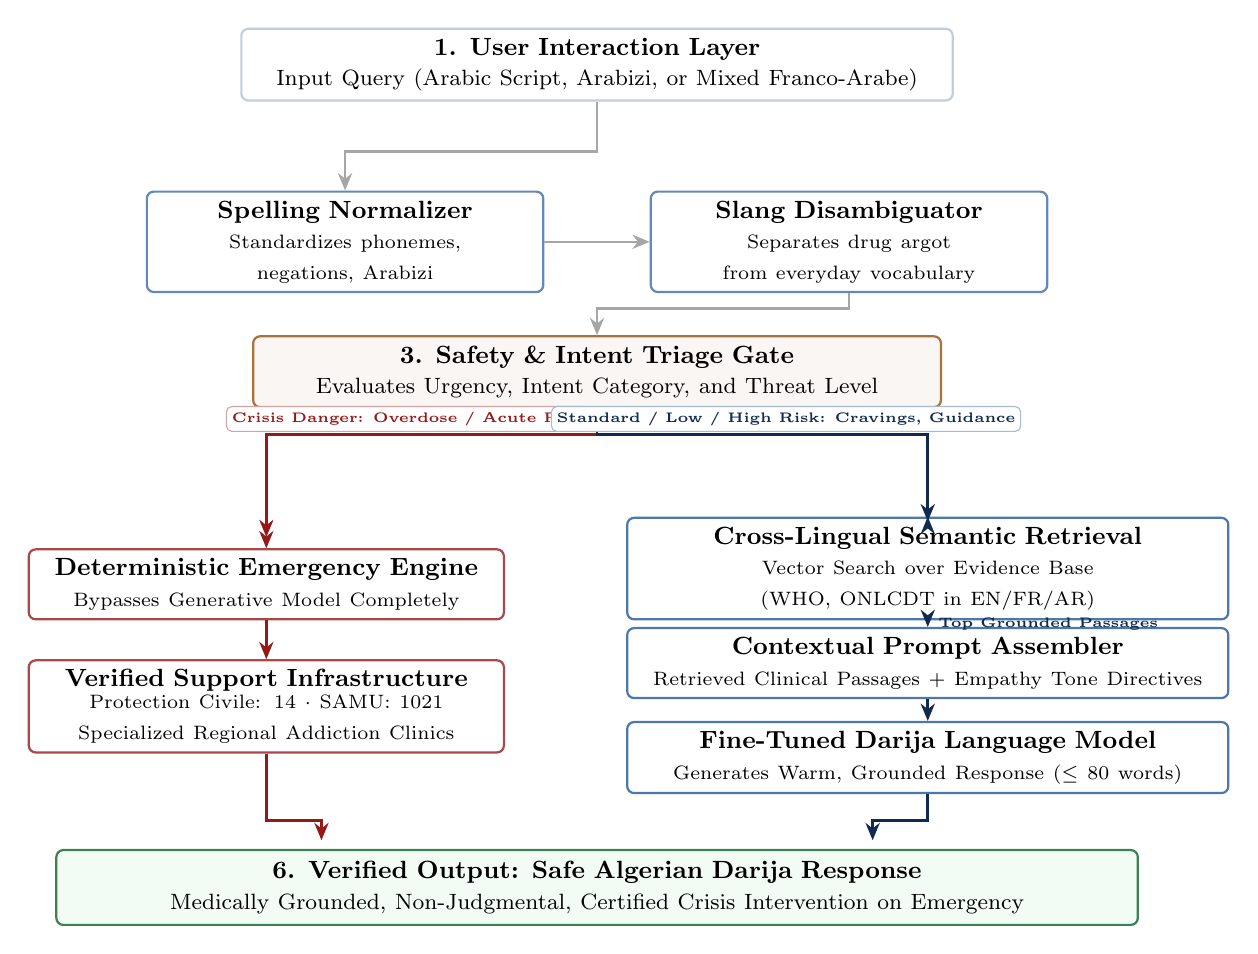
\begin{tikzpicture}

  % 1. Input Node
  \node (input) at (0, 0.5) [flow_box, text width=8.8cm] {
    \textbf{1. User Interaction Layer}\\
    \footnotesize Input Query (Arabic Script, Arabizi, or Mixed Franco-Arabe)
  };

  % 2. Preprocessing Nodes
  \node (norm) at (-3.2, -1.75) [pre_box] {
    \textbf{Spelling Normalizer}\\
    \scriptsize Standardizes phonemes, negations, Arabizi
  };
  \node (slang) at (3.2, -1.75) [pre_box] {
    \textbf{Slang Disambiguator}\\
    \scriptsize Separates drug argot from everyday vocabulary
  };

  % 3. Triage Node
  \node (triage) at (0, -3.4) [triage_box] {
    \textbf{3. Safety \& Intent Triage Gate}\\
    \footnotesize Evaluates Urgency, Intent Category, and Threat Level
  };

  % Subgraph Titles (enclosed in backgrounds)

  % Left Branch: Emergency Intercept
  \node (emerg_eng) at (-4.2, -6.1) [crisis_box] {
    \textbf{Deterministic Emergency Engine}\\
    \scriptsize Bypasses Generative Model Completely
  };
  \node (emerg_hot) at (-4.2, -7.65) [crisis_box] {
    \textbf{Verified Support Infrastructure}\\
    \scriptsize Protection Civile: 14 $\cdot$ SAMU: 1021\\
    \scriptsize Specialized Regional Addiction Clinics
  };

  % Right Branch: Grounded Conversational Engine
  \node (retriever) at (4.2, -5.9) [rag_box] {
    \textbf{Cross-Lingual Semantic Retrieval}\\
    \scriptsize Vector Search over Evidence Base (WHO, ONLCDT in EN/FR/AR)
  };
  \node (prompt_asm) at (4.2, -7.1) [rag_box] {
    \textbf{Contextual Prompt Assembler}\\
    \scriptsize Retrieved Clinical Passages + Empathy Tone Directives
  };
  \node (darija_llm) at (4.2, -8.3) [rag_box] {
    \textbf{Fine-Tuned Darija Language Model}\\
    \scriptsize Generates Warm, Grounded Response ($\le$ 80 words)
  };

  % 6. Output Node
  \node (output) at (0, -9.95) [output_box] {
    \textbf{6. Verified Output: Safe Algerian Darija Response}\\
    \footnotesize Medically Grounded, Non-Judgmental, Certified Crisis Intervention on Emergency
  };

  % Subgraph Backgrounds (fit includes titles!)
  \begin{scope}[on background layer]
  \end{scope}

  % Connectors
  \draw [arr] (input.south) -- (0, -0.6) -| (norm.north);
  \draw [arr] (norm.east) -- (slang.west);
  \draw [arr] (slang.south) |- (0, -2.6) -- (triage.north);

  % Split from Triage with clear spacing
  \draw [danger_arr] (triage.south) -- (0, -4.2) -| (-4.2, -5.5);
  \node at (-2.4, -4.0) [font=\tiny\bfseries\color{darkcrimson}, fill=white, inner sep=2pt, draw=darkcrimson!40, rounded corners=2pt] {Crisis Danger: Overdose / Acute Risk};
  \draw [danger_arr] (-4.2, -5.5) -- (emerg_eng.north);
  \draw [danger_arr] (emerg_eng) -- (emerg_hot);

  \draw [safe_arr] (triage.south) -- (0, -4.2) -| (4.2, -5.3);
  \node at (2.4, -4.0) [font=\tiny\bfseries\color{primarynavy}, fill=white, inner sep=2pt, draw=accentblue!40, rounded corners=2pt] {Standard / Low / High Risk: Cravings, Guidance};
  \draw [safe_arr] (4.2, -5.3) -- (retriever.north);
  \draw [safe_arr] (retriever.south) -- node[right, font=\tiny\bfseries\color{primarynavy}] {Top Grounded Passages} (prompt_asm.north);
  \draw [safe_arr] (prompt_asm) -- (darija_llm);

  % Merge into Output
  \draw [danger_arr] (emerg_hot.south) |- (-4.2, -9.1) -| (-3.5, -9.35);
  \draw [safe_arr] (darija_llm.south) |- (4.2, -9.1) -| (3.5, -9.35);

\end{tikzpicture}
\end{center}

\pagebreak

% ==============================================================================
% PAGE 2: END-TO-END DATA DELIVERY PIPELINE
% ==============================================================================

\noindent{\large\bfseries\color{primarynavy} 2. The End-to-End Data Delivery Pipeline}
\vspace{1.5mm}

\noindent Medical facts are written in formal French and English inside long health reports (WHO, Algerian ONLCDT), while users ask questions in colloquial Algerian Darija, Arabizi, and street slang. The data delivery pipeline is the step-by-step factory line that connects both worlds: it breaks down complex medical guides, cleans real-world language, verifies safety, and powers the AI assistant without translation errors or hallucinations.

\vspace{2.5mm}
\noindent{\normalsize\bfseries\color{accentblue} 2.1 Visual Pipeline Process Map}
\vspace{1.5mm}

\begin{center}
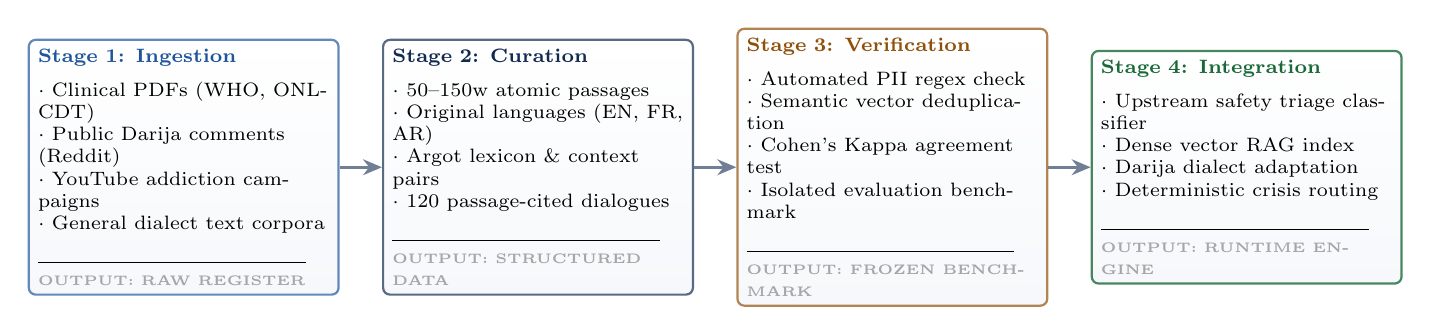
\begin{tikzpicture}[
  stepbox/.style = {base, draw=slateborder, fill=white, text width=3.7cm, minimum height=2.4cm, font=\scriptsize, align=left, top color=white, bottom color=slatebg},
  steparrow/.style = {-{Stealth[length=2.4mm, width=2.0mm]}, line width=1.1pt, color=primarynavy!60}
]

  % Stage 1
  \node (s1) at (0, 0) [stepbox, draw=accentblue!70] {
    \textbf{\color{accentblue} Stage 1: Ingestion}\\[1.5mm]
    $\cdot$ Clinical PDFs (WHO, ONLCDT)\\
    $\cdot$ Public Darija comments (Reddit)\\
    $\cdot$ YouTube addiction campaigns\\
    $\cdot$ General dialect text corpora\\[1.5mm]
    \rule{3.4cm}{0.3pt}\\
    {\tiny\bfseries\color{gray!70} OUTPUT: RAW REGISTER}
  };

  % Stage 2
  \node (s2) at (4.5, 0) [stepbox, draw=primarynavy!70] {
    \textbf{\color{primarynavy} Stage 2: Curation}\\[1.5mm]
    $\cdot$ 50--150w atomic passages\\
    $\cdot$ Original languages (EN, FR, AR)\\
    $\cdot$ Argot lexicon \& context pairs\\
    $\cdot$ 120 passage-cited dialogues\\[1.5mm]
    \rule{3.4cm}{0.3pt}\\
    {\tiny\bfseries\color{gray!70} OUTPUT: STRUCTURED DATA}
  };

  % Stage 3
  \node (s3) at (9.0, 0) [stepbox, draw=amberbrown!70] {
    \textbf{\color{amberbrown} Stage 3: Verification}\\[1.5mm]
    $\cdot$ Automated PII regex check\\
    $\cdot$ Semantic vector deduplication\\
    $\cdot$ Cohen's Kappa agreement test\\
    $\cdot$ Isolated evaluation benchmark\\[1.5mm]
    \rule{3.4cm}{0.3pt}\\
    {\tiny\bfseries\color{gray!70} OUTPUT: FROZEN BENCHMARK}
  };

  % Stage 4
  \node (s4) at (13.5, 0) [stepbox, draw=forestgreen!80] {
    \textbf{\color{forestgreen} Stage 4: Integration}\\[1.5mm]
    $\cdot$ Upstream safety triage classifier\\
    $\cdot$ Dense vector RAG index\\
    $\cdot$ Darija dialect adaptation\\
    $\cdot$ Deterministic crisis routing\\[1.5mm]
    \rule{3.4cm}{0.3pt}\\
    {\tiny\bfseries\color{gray!70} OUTPUT: RUNTIME ENGINE}
  };

  % Arrows between stages
  \draw [steparrow] (s1.east) -- (s2.west);
  \draw [steparrow] (s2.east) -- (s3.west);
  \draw [steparrow] (s3.east) -- (s4.west);

\end{tikzpicture}
\end{center}

\vspace{2mm}
\noindent{\normalsize\bfseries\color{accentblue} 2.2 Operational Principles of the Pipeline Stages}
\vspace{1mm}

\begin{enumerate}\itemsep 1.0mm
  \item \textbf{Stage 1: Collect Raw Data (Ingestion).} We collect two things: (1) official health guides from WHO and the Algerian Ministry of Health to get verified medical facts, and (2) public YouTube and Reddit comments to see how Algerians actually speak and use drug slang.
  \item \textbf{Stage 2: Slice and Structure (Curation).} We cut long PDFs into short, standalone 50--150 word notes (kept in English, French, and Arabic). Then we build a slang dictionary (to understand words with double meanings) and write 120 practice dialogues where every answer cites a specific medical note.
  \item \textbf{Stage 3: Check and Filter (Quality Gate).} Before training, we run an automated script to erase any personal names or phone numbers, use vector similarity to delete duplicate advice, and have two teammates label the same messages to prove our labels are reliable.
  \item \textbf{Stage 4: Power the System (Integration).} Each clean dataset is plugged into its component: labeled messages train the Emergency Triage Gate, medical notes feed the RAG search database, and practice dialogues teach the model to speak warm, natural Darija.
\end{enumerate}

\vspace{2mm}
\noindent{\normalsize\bfseries\color{accentblue} 2.3 Concrete Walkthrough: Lifecycle of a Medical Fact}
\vspace{1.5mm}

\noindent\begin{tabularx}{\textwidth}{lp{3.5cm}X}
\toprule
\textbf{Pipeline Phase} & \textbf{Operational Action} & \textbf{Concrete System Implementation} \\
\midrule
\textbf{1. Ingestion} & Source Document Intake & Official WHO ASSIST Self-Help Guide acquired (60-page PDF manual in English). \\
\addlinespace[1.2mm]
\textbf{2. Curation} & Passage Atomization & Extract 70-word snippet: \textit{"Cravings typically peak within 15 to 30 minutes; drinking water and changing activities helps."} Preserved in English. \\
\addlinespace[1.2mm]
\textbf{3. Quality Gate} & Validation \& Dedup & Automated validator enforces schema compliance, confirms no duplicate exists across Algerian reports, and issues a persistent identifier. \\
\addlinespace[1.2mm]
\textbf{4. Integration} & Multilingual Indexing & Snippet is vectorized using multilingual dense sentence embeddings and stored in the evidence knowledge base. \\
\addlinespace[1.2mm]
\textbf{Live Runtime} & Dialect Query \& Grounded Generation & 
User query: \RL{\arabicfont واش ندير كي تجيني رغبة قوية باش نكمي؟}\newline
Retriever surfaces the English WHO snippet; the fine-tuned LLM generates a culturally adapted response: \newline
\RL{\arabicfont الرغبة هادي ديما تفوت في 15 حتى لـ 30 دقيقة، جرب تبدل البلاصة، تشرب الما...} \\
\bottomrule
\end{tabularx}

\pagebreak

% ==============================================================================
% PAGE 3: CORE OPERATING PRINCIPLES & SYSTEM GUARDRAILS
% ==============================================================================

\noindent{\large\bfseries\color{primarynavy} 3. Core Operating Principles \& System Guardrails}
\vspace{2mm}

\noindent To guarantee absolute clinical safety, ethical compliance, and academic rigor, the project establishes four non-negotiable operational principles across all data and modeling phases.

\vspace{2.5mm}

\begin{tcolorbox}[colback=subtleblue!50, colframe=accentblue!60, boxrule=0.6pt, arc=3pt, left=10pt, right=10pt, top=6pt, bottom=6pt]
\textbf{\color{primarynavy} Principle 1: Knowledge Preservation in Source Languages (EN / FR / AR)}\\
\footnotesize Pre-translating institutional clinical guidelines into Darija introduces severe lexical ambiguity and risks generating erroneous medical advice. Raw evidence is preserved in its authentic publication languages. The retrieval layer executes semantic cross-lingual matching, while the generation model translates and contextualizes the facts into natural Darija within the conversation.
\end{tcolorbox}

\vspace{1.5mm}

\begin{tcolorbox}[colback=subtlered!50, colframe=darkcrimson!60, boxrule=0.6pt, arc=3pt, left=10pt, right=10pt, top=6pt, bottom=6pt]
\textbf{\color{darkcrimson} Principle 2: Zero-Hallucination Emergency Protocol (Deterministic Bypass)}\\
\footnotesize Under no circumstances may an acute emergency (e.g., suspected drug overdose, respiratory depression, loss of consciousness, or suicidal intent) be delegated to an open-ended generative language model. The upstream triage classifier immediately diverts crisis queries to pre-verified, deterministic emergency templates providing authenticated Algerian contact numbers (Protection Civile 14, SAMU 1021, and specialized addiction clinics).
\end{tcolorbox}

\vspace{1.5mm}

\begin{tcolorbox}[colback=slatebg, colframe=amberbrown!60, boxrule=0.6pt, arc=3pt, left=10pt, right=10pt, top=6pt, bottom=6pt]
\textbf{\color{amberbrown} Principle 3: Religious Guidance is Strictly Opt-In}\\
\footnotesize While spiritual values represent a meaningful source of recovery motivation for many Algerians, introducing unsolicited religious rhetoric into medical queries can generate moral guilt, increase perceived stigma, and alienate vulnerable individuals. Religious passages are maintained as a segregated taxonomy class and are surfaced \textit{only} when the user explicitly solicits spiritual or moral guidance.
\end{tcolorbox}

\vspace{1.5mm}

\begin{tcolorbox}[colback=subtlegreen!50, colframe=forestgreen!60, boxrule=0.6pt, arc=3pt, left=10pt, right=10pt, top=6pt, bottom=6pt]
\textbf{\color{forestgreen} Principle 4: Strict Factual Grounding and Citation Integrity}\\
\footnotesize Every assistant response in non-emergency interactions must be mathematically constrained to the evidence retrieved from the knowledge base. Assistant turns must stay within an 80-word ceiling, maintain a warm, non-judgmental tone, and cite verified passage identifiers. The model is strictly prohibited from inventing treatment regimens or withdrawal timelines.
\end{tcolorbox}

\vspace{3mm}
\noindent{\normalsize\bfseries\color{accentblue} 3.1 Overview of the Three Core AI Components}
\vspace{1.5mm}

\noindent\begin{tabularx}{\textwidth}{p{3.8cm}p{4.6cm}X}
\toprule
\textbf{Subsystem} & \textbf{Underlying Methodology} & \textbf{System Responsibility} \\
\midrule
\textbf{1. Upstream Safety Triage Gate} & Multi-class discriminative classification (BERT / FastText backbone). & Classifies intent categories and threat levels (\textit{None, Low, High, Crisis}). Diverts life-threatening inputs to certified emergency templates before reaching generative models. \\
\addlinespace[1.5mm]
\textbf{2. Cross-Lingual Semantic RAG} & Multilingual dense vector representations with cosine similarity indexing. & Enables a user query in Darija or Arabizi to accurately retrieve underlying evidence passages authored in English, French, or Standard Arabic without machine translation noise. \\
\addlinespace[1.5mm]
\textbf{3. Fine-Tuned Darija LLM} & Open-weights bilingual LLM adapted on grounded dialogues and dialect corpora. & Synthesizes retrieved evidence into concise ($\le$ 80 words), empathetic, and culturally authentic Algerian Darija, observing agreed spelling norms and medical constraints. \\
\bottomrule
\end{tabularx}

\end{document}
